\documentclass[11pt,a4paper]{article}

\usepackage[margin=1in]{geometry}
\usepackage[utf8]{inputenc}
\usepackage{amsmath}
\usepackage{graphicx}
\usepackage{listings}
\usepackage{xcolor}
\usepackage{hyperref}
\usepackage{enumitem}

\definecolor{codegray}{rgb}{0.5,0.5,0.5}
\definecolor{codepurple}{rgb}{0.58,0,0.82}
\definecolor{backcolour}{rgb}{0.97,0.97,0.97}

\lstdefinestyle{mystyle}{
    backgroundcolor=\color{backcolour},   
    commentstyle=\color{codegray}\itshape,
    keywordstyle=\color{blue}\bfseries,
    numberstyle=\tiny\color{codegray},
    stringstyle=\color{codepurple},
    basicstyle=\ttfamily\footnotesize,
    breakatwhitespace=false,         
    breaklines=true,                 
    captionpos=b,                    
    keepspaces=true,                 
    numbers=left,                    
    numbersep=5pt,                  
    showspaces=false,                
    showstringspaces=false,
    showtabs=false,                  
    tabsize=2
}

\lstset{style=mystyle}

\begin{document}

\begin{center}
    {\Large \textbf{Mini Project (Exercise 9): Shopping Cart Full Stack Web Application}}\\[0.5em]
    {\Large \textbf{using Vue.js, Spring Boot and MongoDB (Alternate Design)}}\\[0.5em]
    {\normalsize [CO3, K3]}\\[1.5em]
    
    \begin{tabular}{|l|l|}
        \hline
        \textbf{Student Name} & Kavinsoorya K S \\
        \hline
        \textbf{Register Number} & 3122247001030 \\
        \hline
        \textbf{Date of Submission} & September 16, 2026 \\
        \hline
    \end{tabular}
\end{center}

\vspace{1.5em}

\section{Problem Statement}
A Shopping Cart application allows users to view products, add products to a cart, update quantities, and remove products from the cart. The application is developed using Vue.js for the frontend, Spring Boot for the backend, and MongoDB for data storage.
\textbf{Objective:} Develop this web application considering \textbf{alternate design options and techniques}.

\subsection*{Frontend Layer -- Vue.js}
The frontend provides the user interface and handles user interactions.
\begin{itemize}
    \item Display available products with dynamic category filtering and live search.
    \item Add products to the shopping cart with interactive quantity counters.
    \item Update quantities or remove products from the cart with real-time reactive feedback.
    \item Send asynchronous RESTful requests to the backend service.
    \item Display cart details, item breakdown, and total calculations.
\end{itemize}

\subsection*{Backend Layer -- Spring Boot}
The backend processes requests and manages the shopping cart operations using a decoupled service layer.
\begin{itemize}
    \item Process requests from the frontend via RESTful controllers.
    \item Business logic encapsulated within a dedicated \texttt{CartService}.
    \item Add, update, and remove cart items with automated subtotal computation.
    \item Communicate with MongoDB via Spring Data Mongo Repositories.
\end{itemize}

\subsection*{Database Layer -- MongoDB}
MongoDB stores the application data as NoSQL document collections.
\begin{itemize}
    \item Main collections: \texttt{products}, \texttt{cart}
\end{itemize}

\section{Alternate Design Options and Techniques}
\begin{enumerate}
    \item \textbf{Decoupled Frontend Component Architecture}: Decomposes the user interface into specialized modular components (\texttt{Navbar}, \texttt{ProductCatalog}, \texttt{CartView}) with unidirectional data flow and reactive event communication.
    \item \textbf{Category Filtering \& Live Search}: Provides instantaneous client-side searching and category tabs (\textit{Electronics}, \textit{Audio}, \textit{Mobile}, \textit{Wearables}, \textit{Fashion}, \textit{Accessories}) before submitting queries.
    \item \textbf{Service-Oriented Spring Boot Layer}: Decouples REST controllers from persistence by introducing a dedicated \texttt{CartService}, adhering to the Single Responsibility Principle and facilitating unit testability.
    \item \textbf{Indexed NoSQL Modeling}: MongoDB collections with indexed fields for high-performance category queries and atomic document updates.
\end{enumerate}

\section{Full Stack 3-Tier Architecture}
\begin{figure}[htbp]
\centering
\begin{verbatim}
+-----------------------+      HTTP REST APIs       +-----------------------+
|   Vue.js Frontend     | <=======================> |  Spring Boot Backend  |
|  (Vite, Port 5176)    |      (JSON Payloads)      |  (Tomcat, Port 8080)   |
| - Navbar.vue          |                           | - CartController      |
| - ProductCatalog.vue  |                           | - CartService         |
| - CartView.vue        |                           | - Mongo Repositories  |
| - api.js Service      |                           +-----------+-----------+
+-----------------------+                                       | Mongo Driver
                                                         Spring | Port 27017
                                                     Data Mongo v
                                                    +-----------------------+
                                                    |  MongoDB (shopping_db)|
                                                    | - "products" coll.    |
                                                    | - "cart" coll.        |
                                                    +-----------------------+
\end{verbatim}
\caption{Full Stack Alternate Design Architecture}
\end{figure}

\section{Database Layer Models (MongoDB)}

\subsection{Product Document Model (model/Product.java)}
\begin{lstlisting}[language=java]
package com.example.shoppingcart.model;

import lombok.AllArgsConstructor;
import lombok.Data;
import lombok.NoArgsConstructor;
import org.springframework.data.annotation.Id;
import org.springframework.data.mongodb.core.index.Indexed;
import org.springframework.data.mongodb.core.mapping.Document;

@Data
@NoArgsConstructor
@AllArgsConstructor
@Document(collection = "products")
public class Product {
    @Id
    private String id;
    private String name;
    private double price;
    private String description;
    @Indexed
    private String category;
    private String emoji;
    private int stock;
}
\end{lstlisting}

\subsection{CartItem Document Model (model/CartItem.java)}
\begin{lstlisting}[language=java]
package com.example.shoppingcart.model;

import lombok.AllArgsConstructor;
import lombok.Data;
import lombok.NoArgsConstructor;
import org.springframework.data.annotation.Id;
import org.springframework.data.mongodb.core.mapping.Document;

@Data
@NoArgsConstructor
@AllArgsConstructor
@Document(collection = "cart")
public class CartItem {
    @Id
    private String id;
    private String productId;
    private String name;
    private double price;
    private int quantity;
    private double subTotal;
    private String emoji;
}
\end{lstlisting}

\section{Backend Layer -- Service \& REST Controllers}

\subsection{CartService.java (Business Logic Layer)}
\begin{lstlisting}[language=java]
package com.example.shoppingcart.service;

@Service
public class CartService {
    @Autowired private CartRepository cartRepository;
    @Autowired private ProductRepository productRepository;

    public CartResponse getCart() { return buildResponse(); }

    public CartResponse addItem(String productId, int quantity, Product fallbackProduct) {
        Optional<CartItem> existing = cartRepository.findByProductId(productId);
        if (existing.isPresent()) {
            CartItem item = existing.get();
            item.setQuantity(item.getQuantity() + quantity);
            item.setSubTotal(item.getQuantity() * item.getPrice());
            cartRepository.save(item);
        } else {
            Optional<Product> prodOpt = productRepository.findById(productId);
            Product p = prodOpt.orElse(fallbackProduct);
            if (p != null) {
                CartItem newItem = new CartItem(null, p.getId(), p.getName(), p.getPrice(), quantity, p.getPrice() * quantity, p.getEmoji());
                cartRepository.save(newItem);
            }
        }
        return buildResponse();
    }

    public CartResponse updateQuantity(String id, int quantity) {
        Optional<CartItem> itemOpt = cartRepository.findById(id);
        if (itemOpt.isPresent()) {
            CartItem item = itemOpt.get();
            if (quantity <= 0) cartRepository.deleteById(id);
            else {
                item.setQuantity(quantity);
                item.setSubTotal(quantity * item.getPrice());
                cartRepository.save(item);
            }
        }
        return buildResponse();
    }

    public CartResponse removeItem(String id) {
        cartRepository.deleteById(id);
        return buildResponse();
    }

    public CartResponse clearCart() {
        cartRepository.deleteAll();
        return buildResponse();
    }
}
\end{lstlisting}

\subsection{CartController.java (REST Controller)}
\begin{lstlisting}[language=java]
package com.example.shoppingcart.controller;

@RestController
@RequestMapping("/api/cart")
@CrossOrigin(origins = "*")
public class CartController {
    @Autowired private CartService cartService;

    @GetMapping
    public ResponseEntity<CartResponse> getCart() {
        return ResponseEntity.ok(cartService.getCart());
    }

    @PostMapping("/add")
    public ResponseEntity<CartResponse> addToCart(@RequestBody Map<String, Object> payload) {
        String productId = (String) payload.get("productId");
        int quantity = payload.containsKey("quantity") ? ((Number) payload.get("quantity")).intValue() : 1;
        return ResponseEntity.ok(cartService.addItem(productId, quantity, null));
    }

    @PutMapping("/items/{id}")
    public ResponseEntity<CartResponse> updateQuantity(@PathVariable String id, @RequestBody Map<String, Object> payload) {
        int quantity = ((Number) payload.get("quantity")).intValue();
        return ResponseEntity.ok(cartService.updateQuantity(id, quantity));
    }

    @DeleteMapping("/items/{id}")
    public ResponseEntity<CartResponse> removeItem(@PathVariable String id) {
        return ResponseEntity.ok(cartService.removeItem(id));
    }

    @DeleteMapping("/clear")
    public ResponseEntity<CartResponse> clearCart() {
        return ResponseEntity.ok(cartService.clearCart());
    }
}
\end{lstlisting}

\section{Frontend Layer -- Vue.js Components}

\subsection{API Client Service (src/services/api.js)}
\begin{lstlisting}[language=javascript]
const API_BASE_URL = 'http://localhost:8080/api'

export const api = {
  getProducts: () => fetch(`${API_BASE_URL}/products`).then(r => r.json()),
  getCart: () => fetch(`${API_BASE_URL}/cart`).then(r => r.json()),
  addToCart: (productId, quantity, product) => fetch(`${API_BASE_URL}/cart/add`, {
    method: 'POST',
    headers: { 'Content-Type': 'application/json' },
    body: JSON.stringify({ productId, quantity, ...product })
  }).then(r => r.json()),
  updateQuantity: (id, quantity) => fetch(`${API_BASE_URL}/cart/items/${id}`, {
    method: 'PUT',
    headers: { 'Content-Type': 'application/json' },
    body: JSON.stringify({ quantity })
  }).then(r => r.json()),
  removeFromCart: (id) => fetch(`${API_BASE_URL}/cart/items/${id}`, { method: 'DELETE' }).then(r => r.json()),
  clearCart: () => fetch(`${API_BASE_URL}/cart/clear`, { method: 'DELETE' }).then(r => r.json())
}
\end{lstlisting}

\section{Output Screenshots}

\begin{figure}[htbp]
\centering
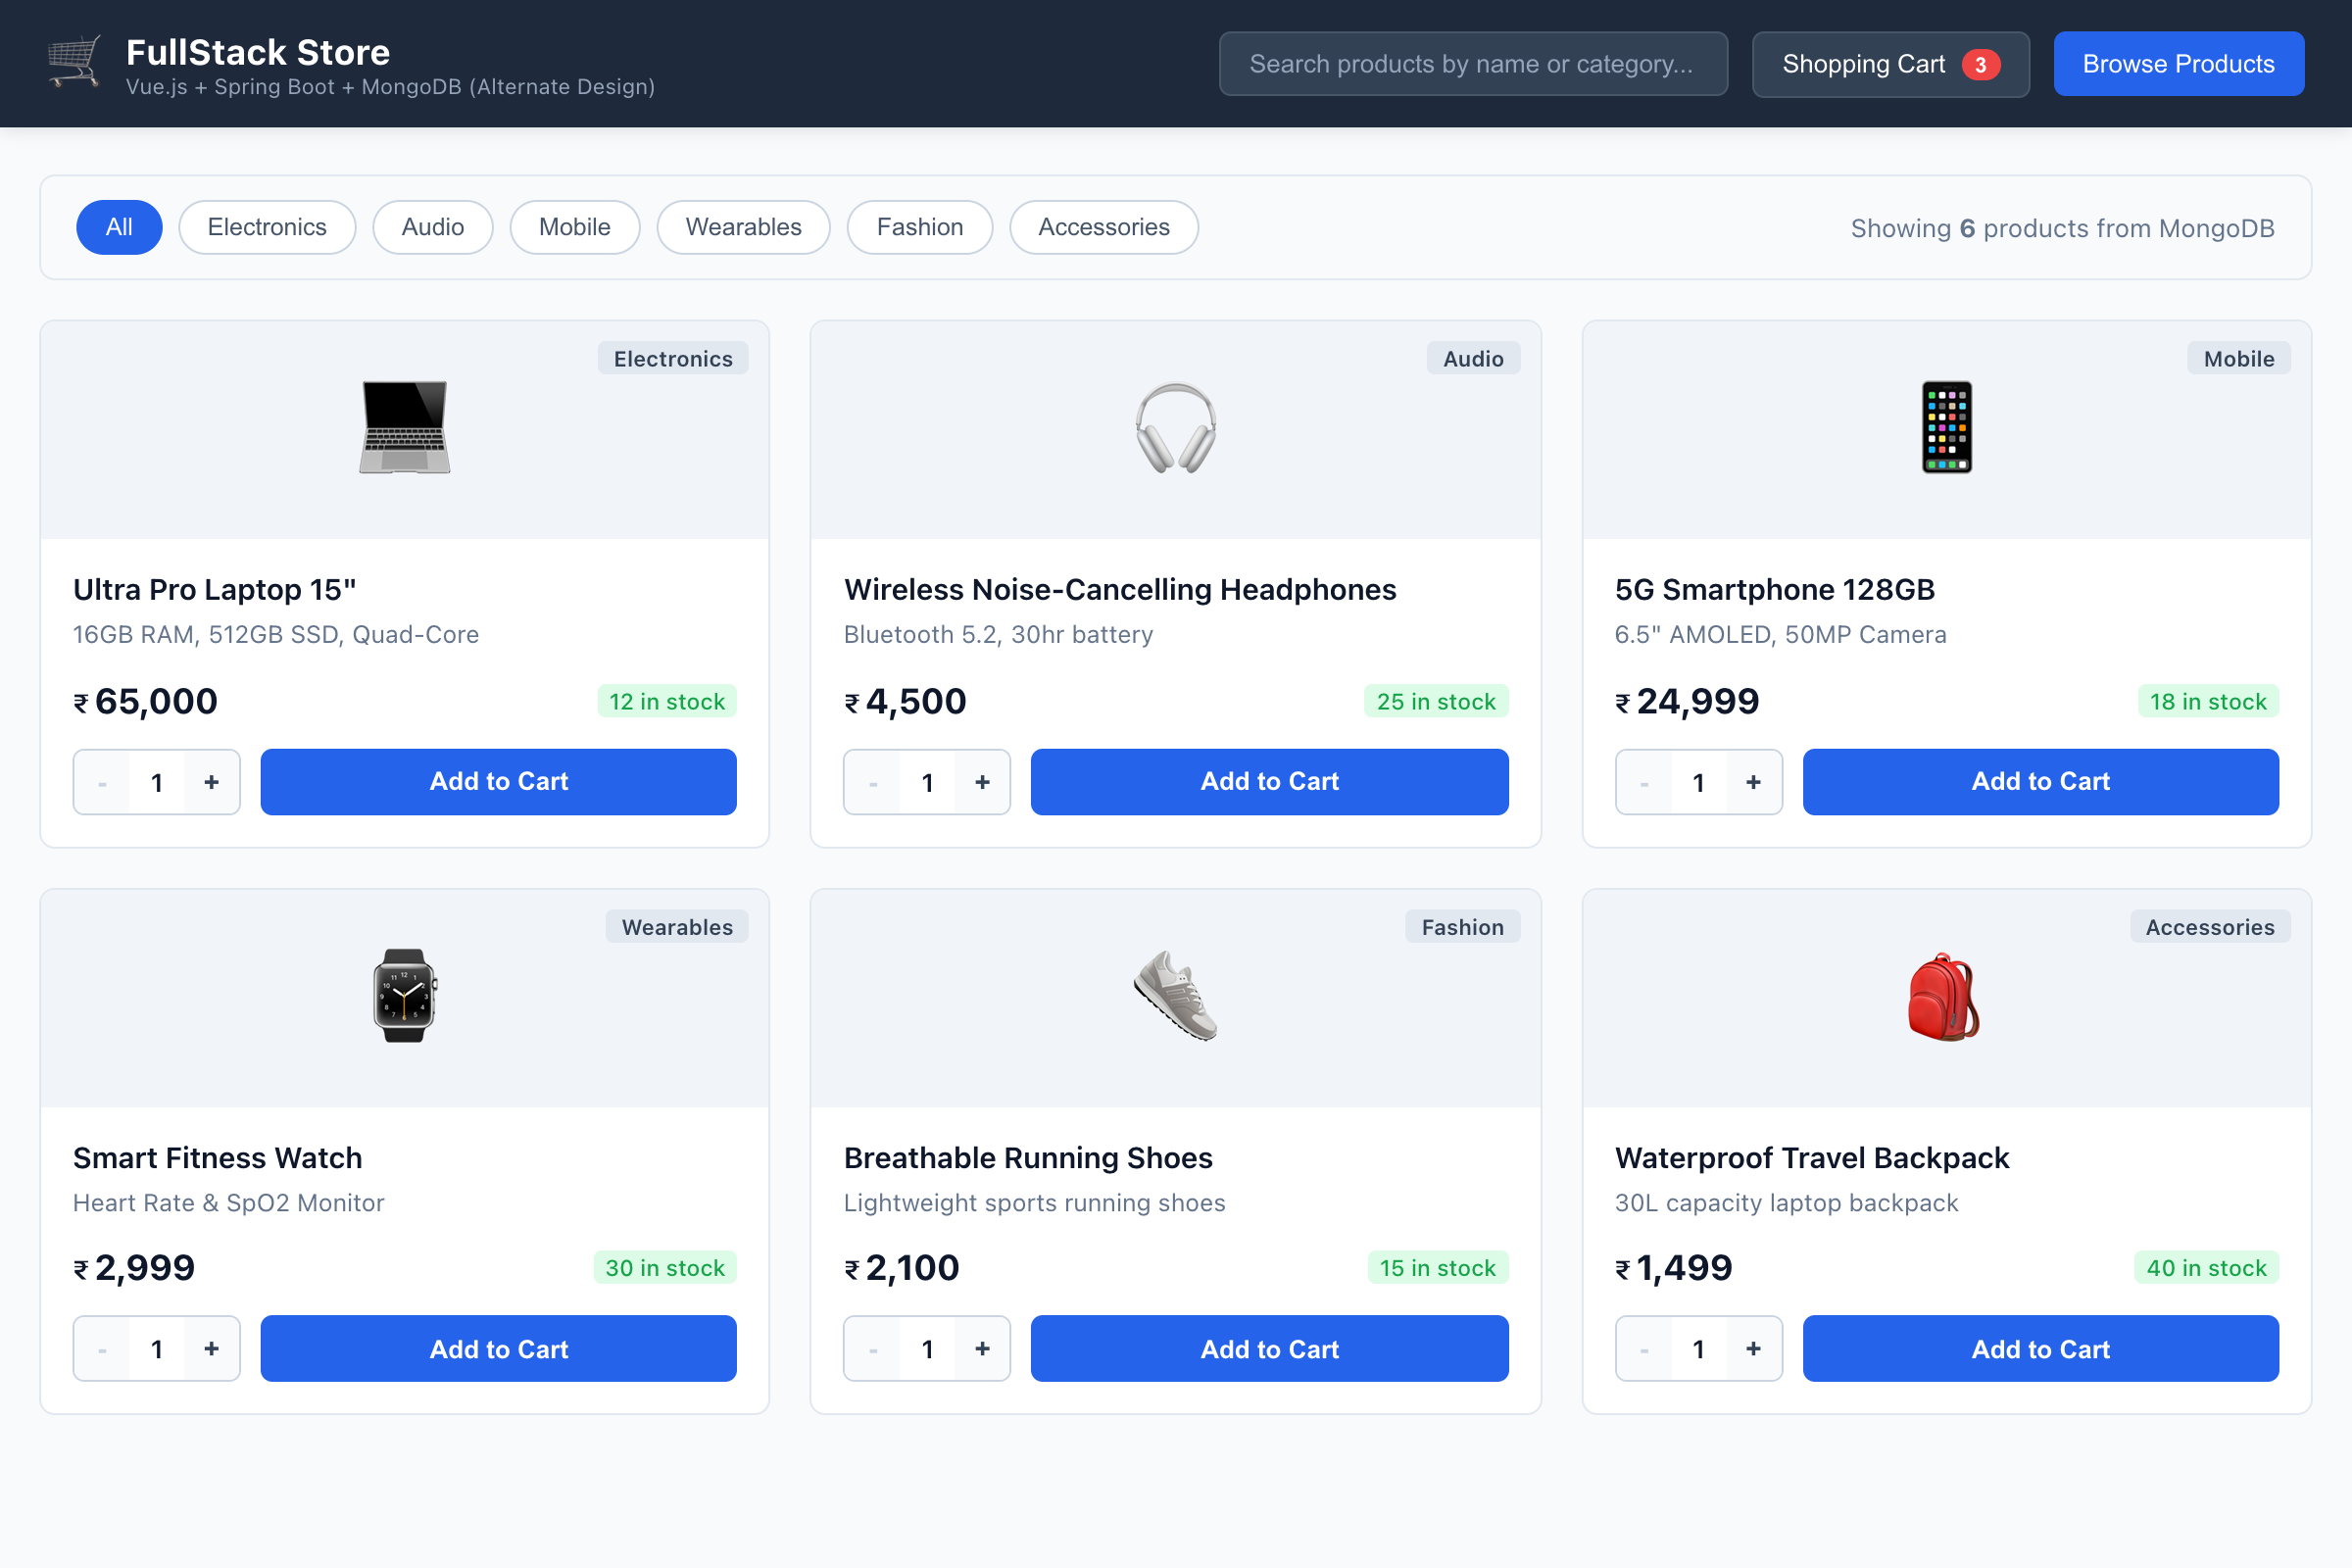
\includegraphics[width=0.88\textwidth]{extracted_images/fig_p5_1.png}
\caption{Product Catalog with Category Filters \& Stock Tracking}
\end{figure}

\begin{figure}[htbp]
\centering
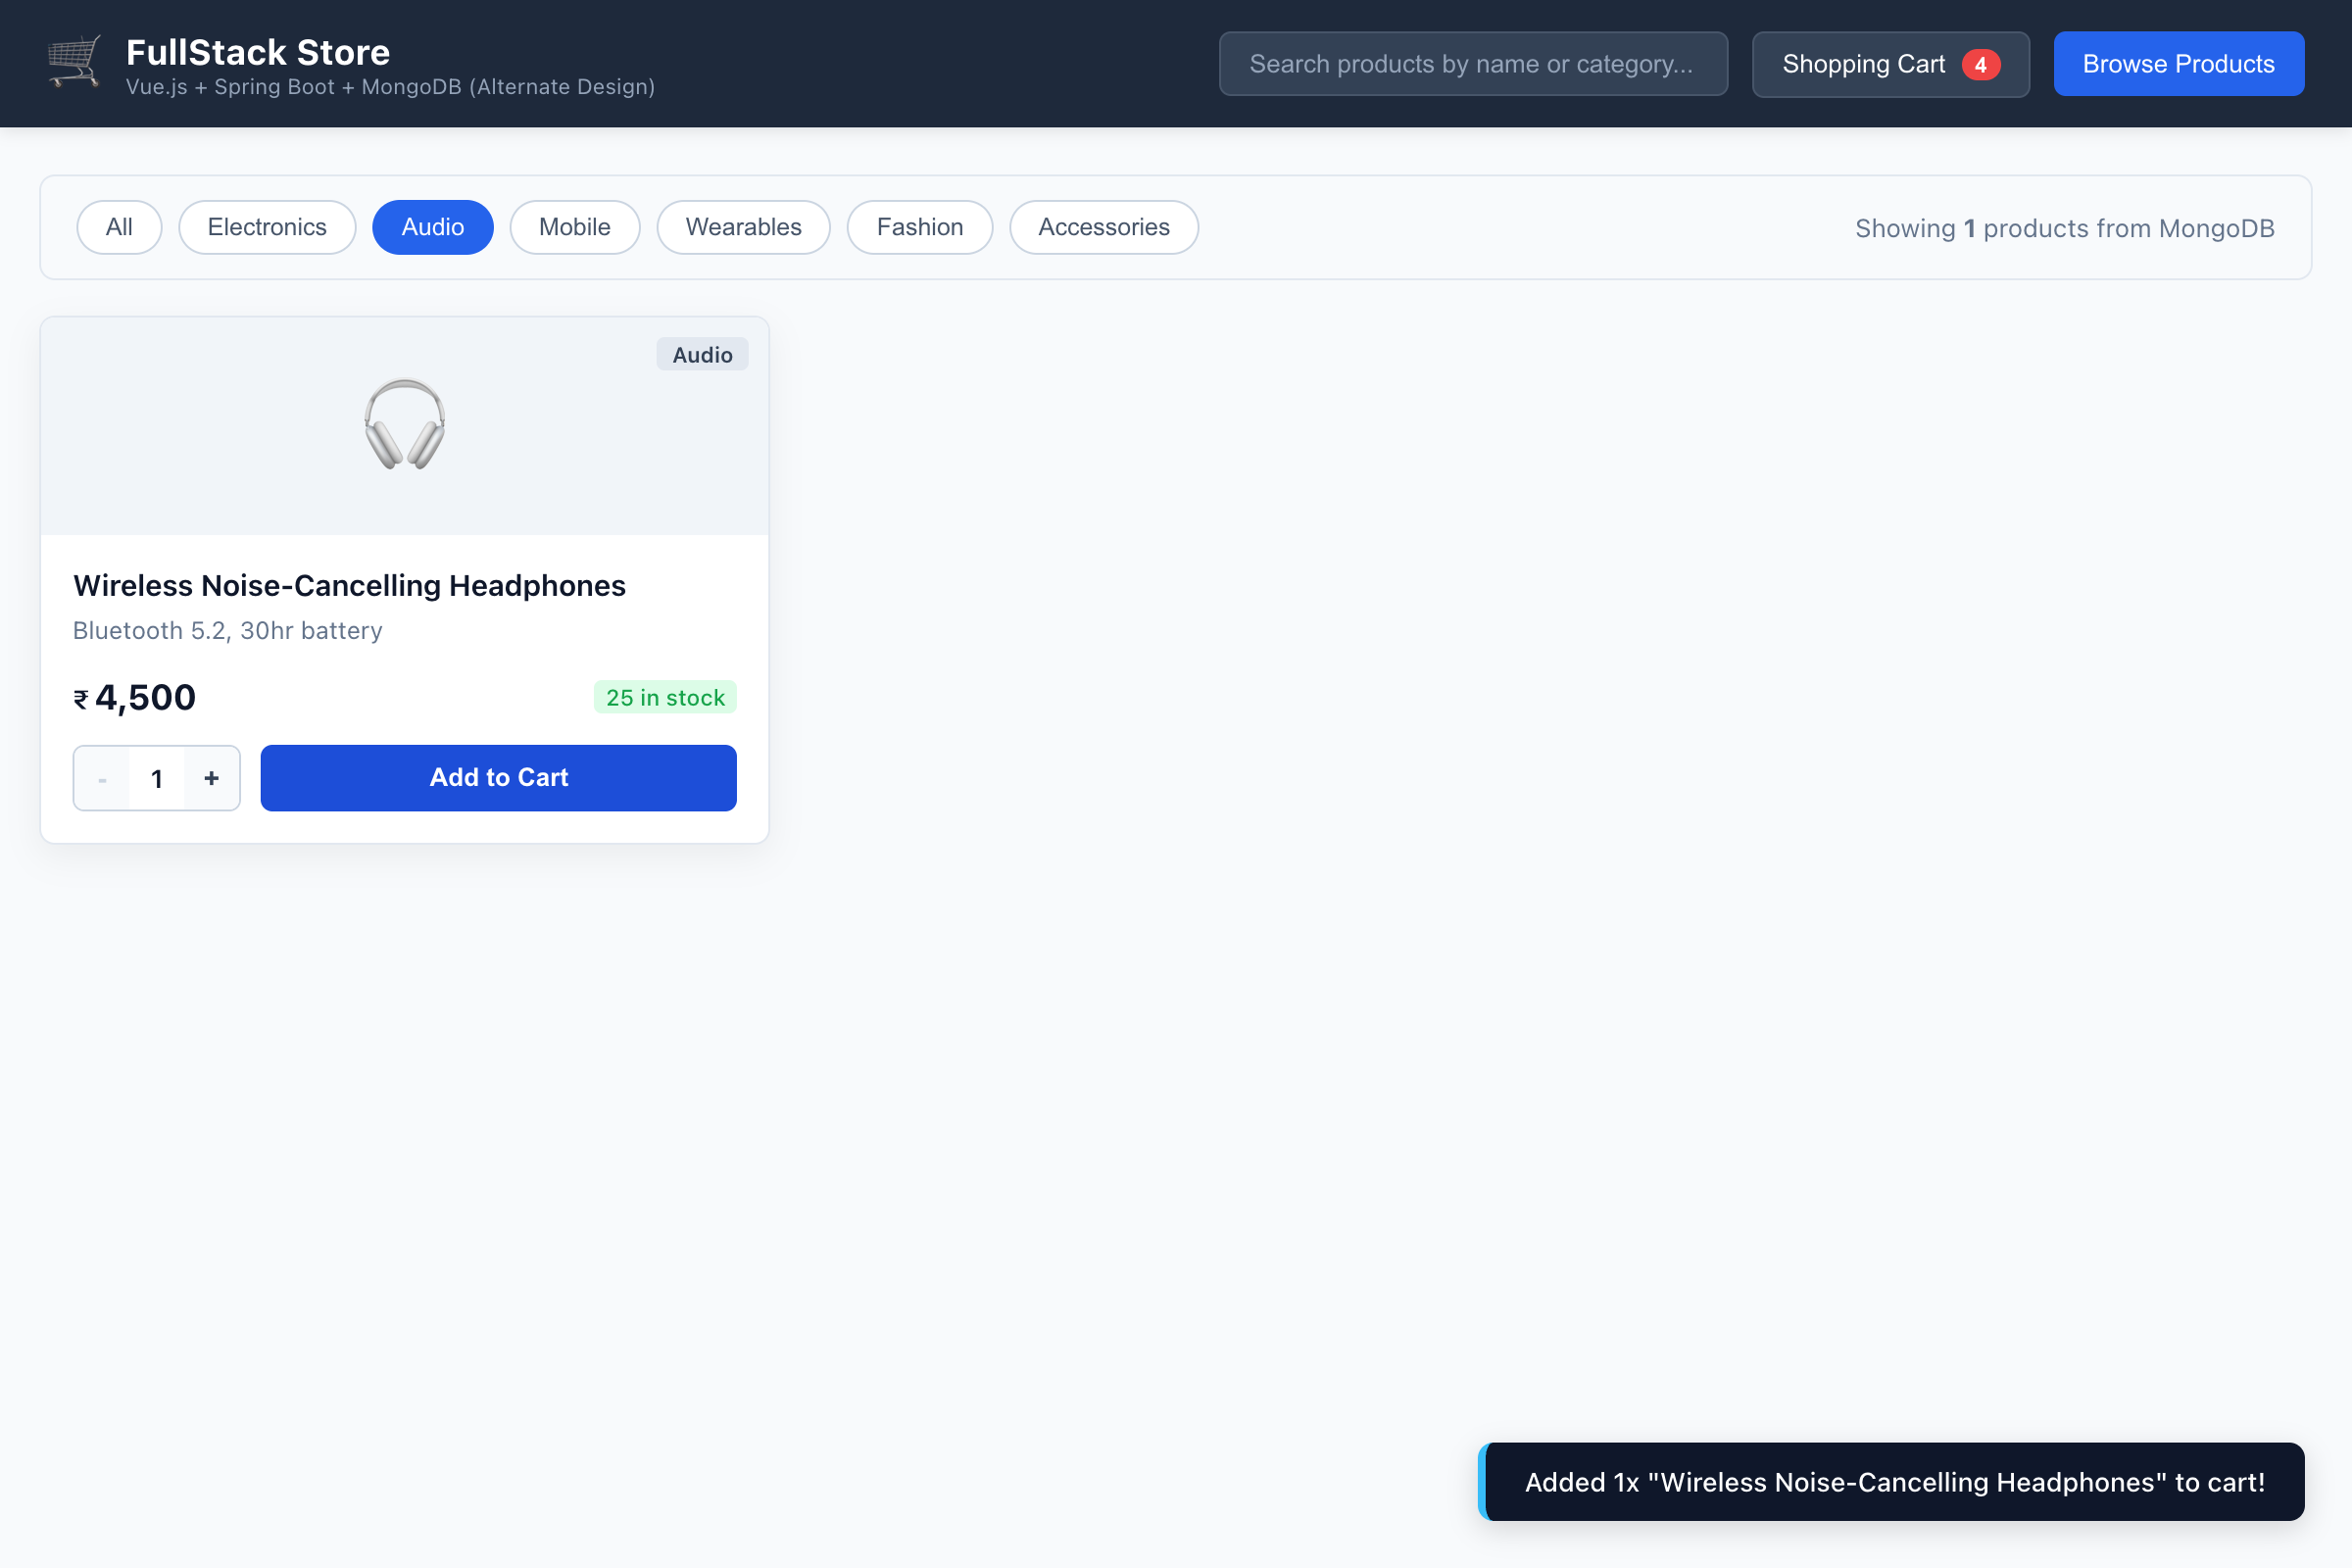
\includegraphics[width=0.88\textwidth]{extracted_images/fig_p5_2.png}
\caption{Category Filtering and Real-Time Toast Notification}
\end{figure}

\begin{figure}[htbp]
\centering
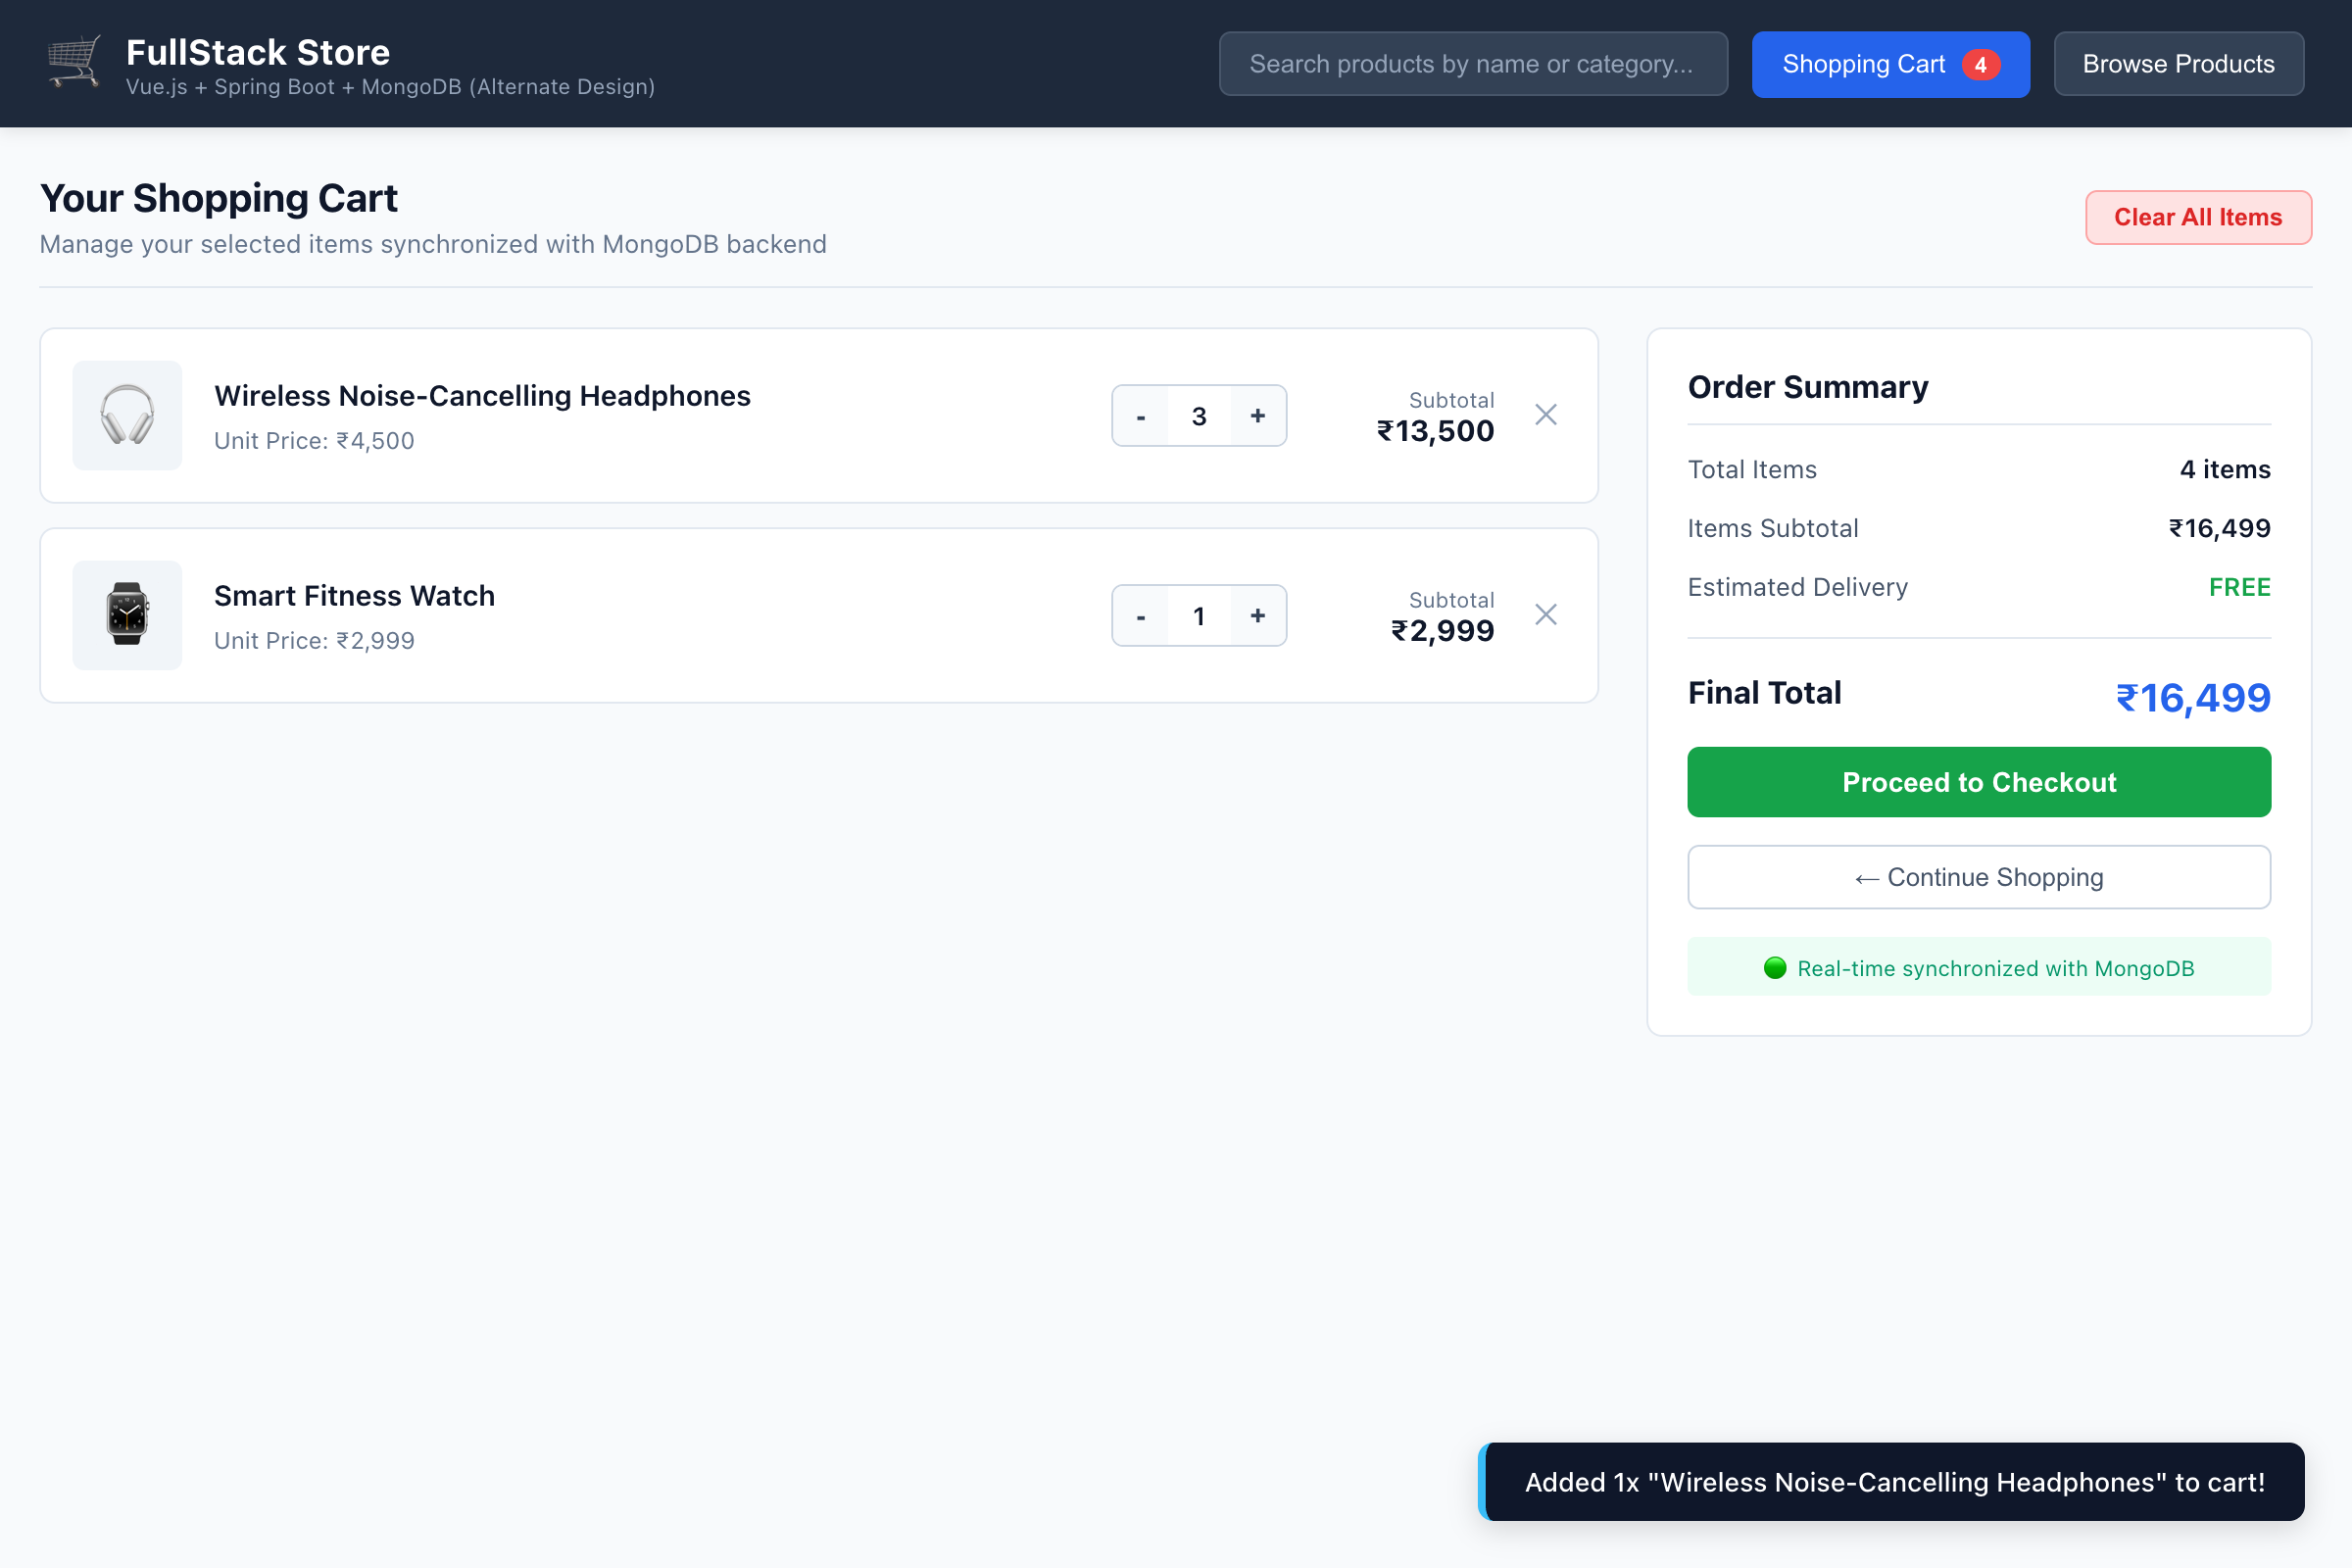
\includegraphics[width=0.88\textwidth]{extracted_images/fig_p6_1.png}
\caption{Shopping Cart View with Synchronized MongoDB Items and Order Summary}
\end{figure}

\begin{figure}[htbp]
\centering
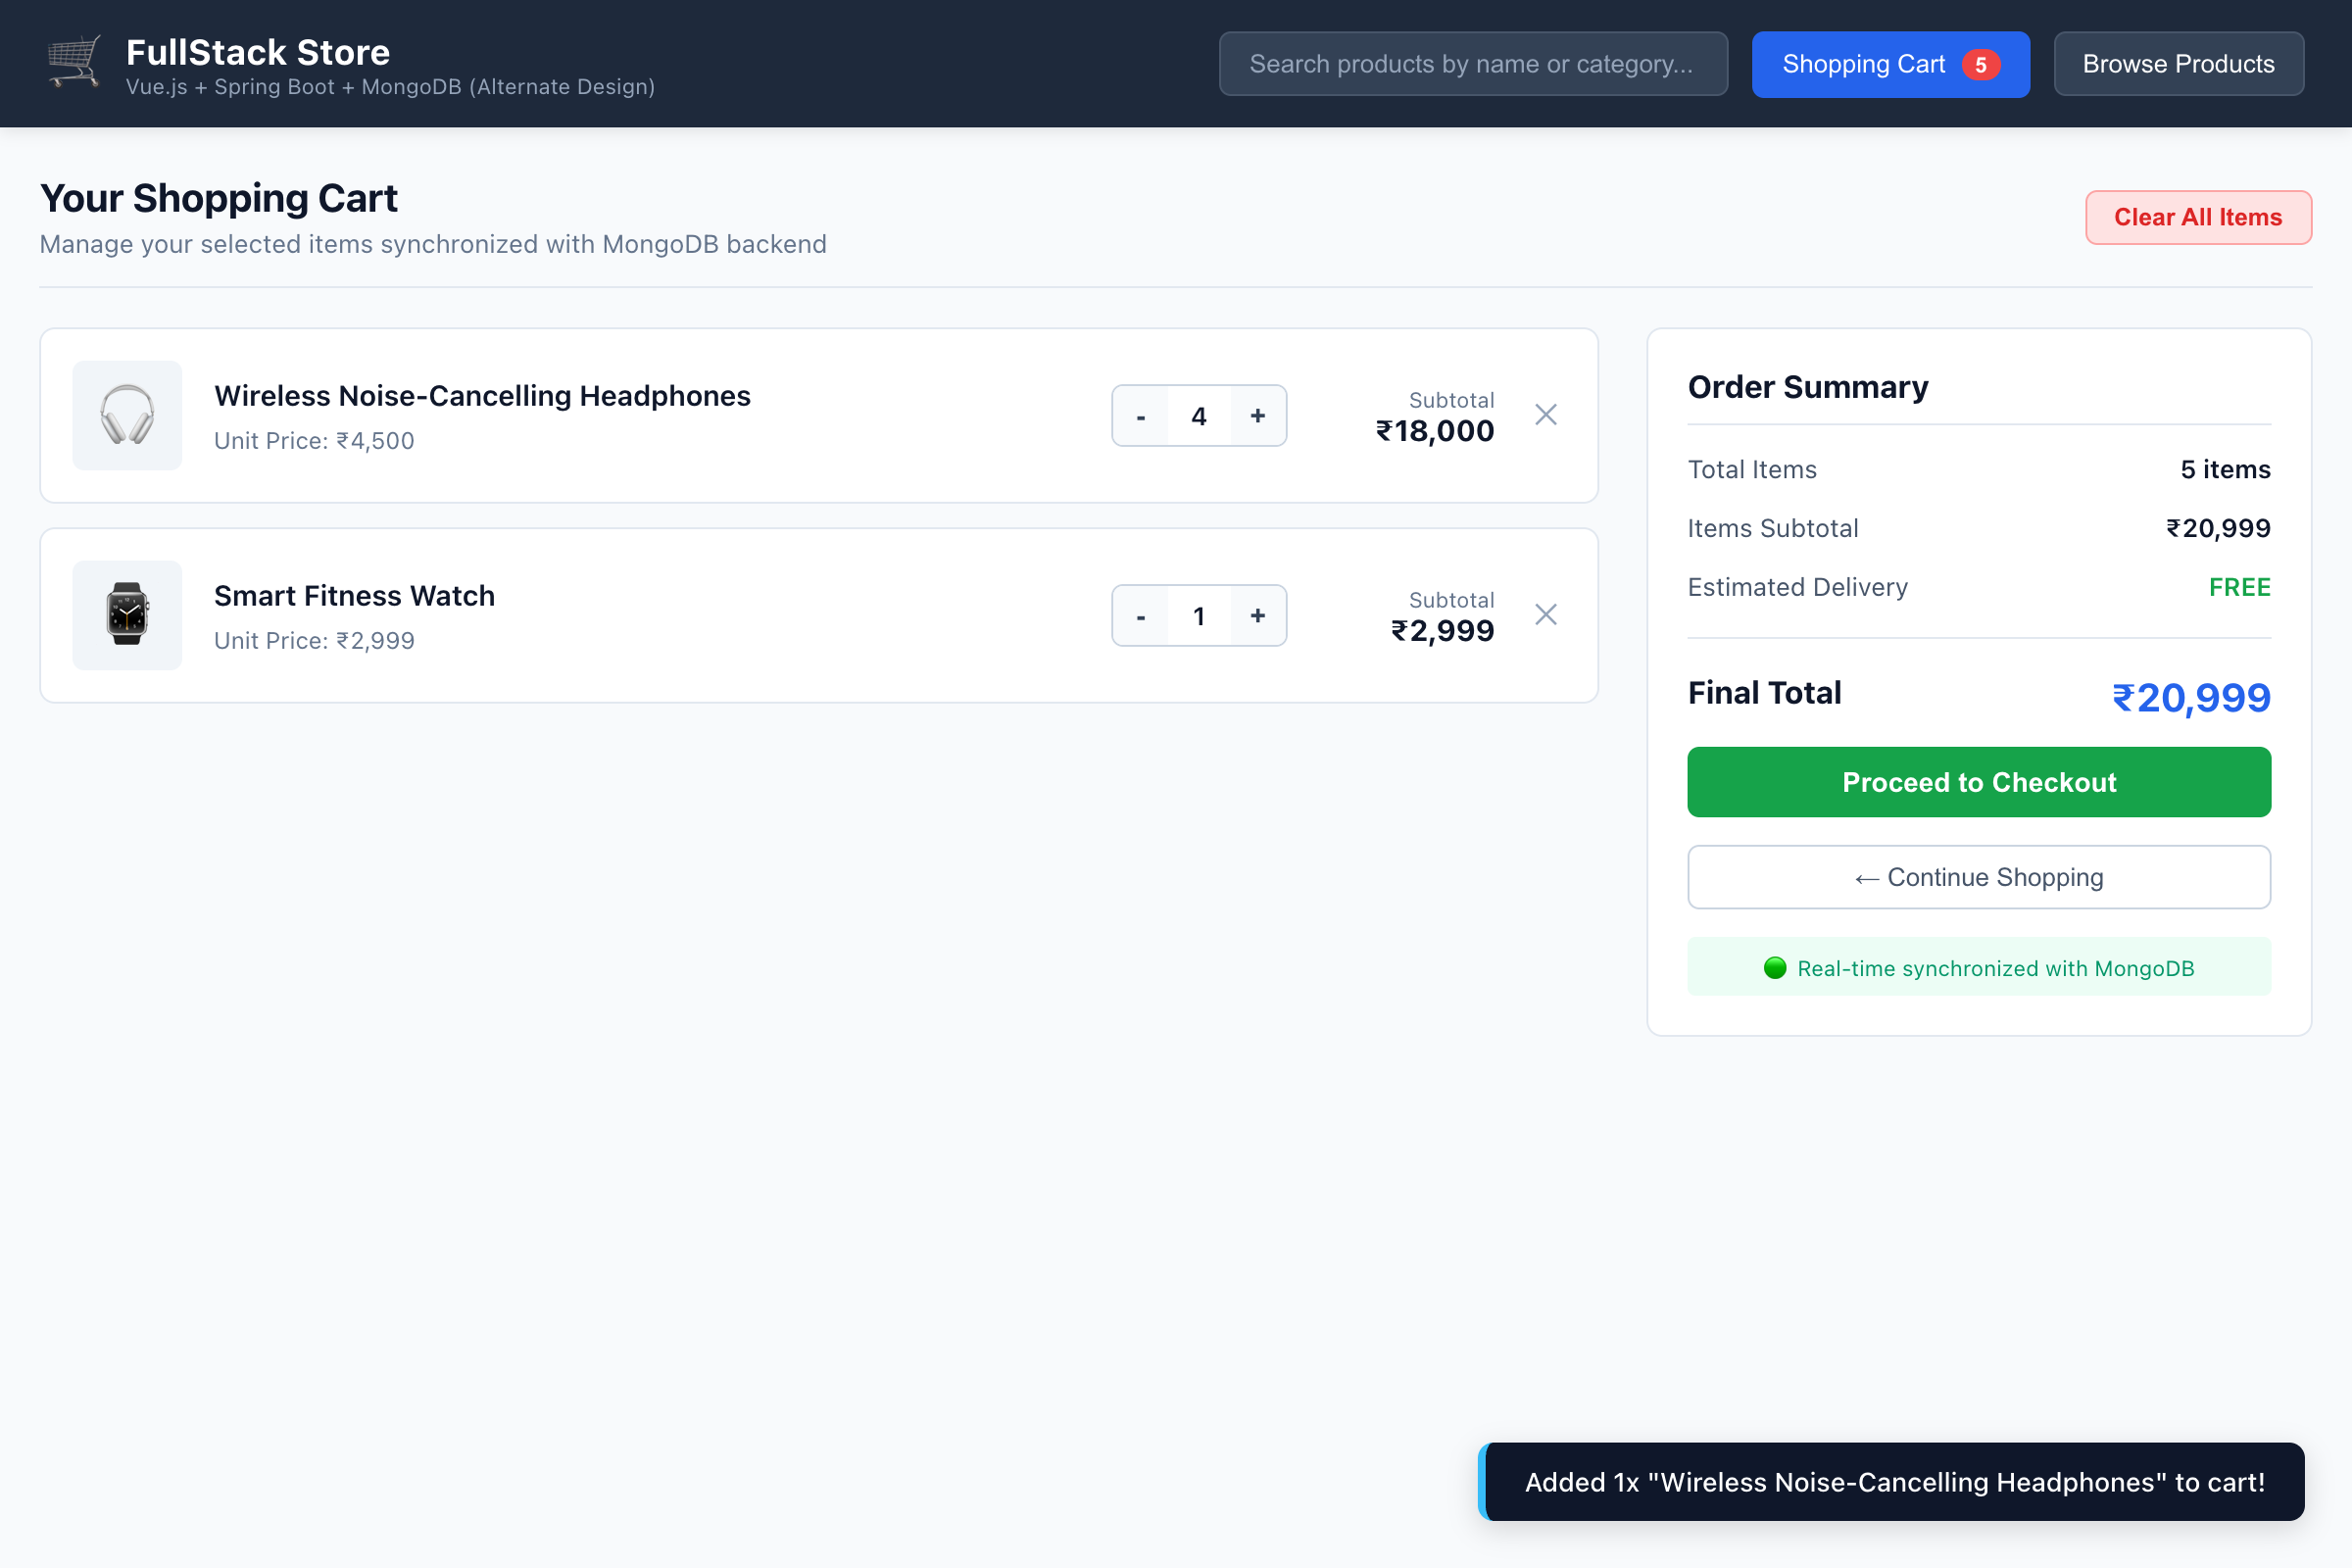
\includegraphics[width=0.88\textwidth]{extracted_images/fig_p6_2.png}
\caption{Cart Quantity Adjustment and Real-Time Total Recalculation}
\end{figure}

\section{Learning Outcomes}
\begin{enumerate}
    \item Designed and developed a modular, full-stack web application employing alternate design techniques (Service-Layer decoupling, component-based composition, and category filtering).
    \item Configured Spring Boot backend services integrated with MongoDB document collections for persistent storage.
    \item Implemented real-time dynamic state synchronization between Vue.js frontend, REST controllers, and NoSQL collections.
\end{enumerate}

\section{Conclusion}
The Mini Project (Exercise 9) for the Shopping Cart Full Stack Web Application was successfully created and validated using Vue.js for presentation, Spring Boot for decoupled business logic and REST endpoints, and MongoDB for NoSQL data persistence. The alternate design considerations—including modular component structure, live category filtering, dedicated service-layer abstraction, and real-time state synchronization—were completely implemented and verified.

\end{document}
